\chapter{Anhang}
\section{Screenshots der Webapplikation}
\subsection{Willkommensseite}
\begin{figure}[H]
  \centering
  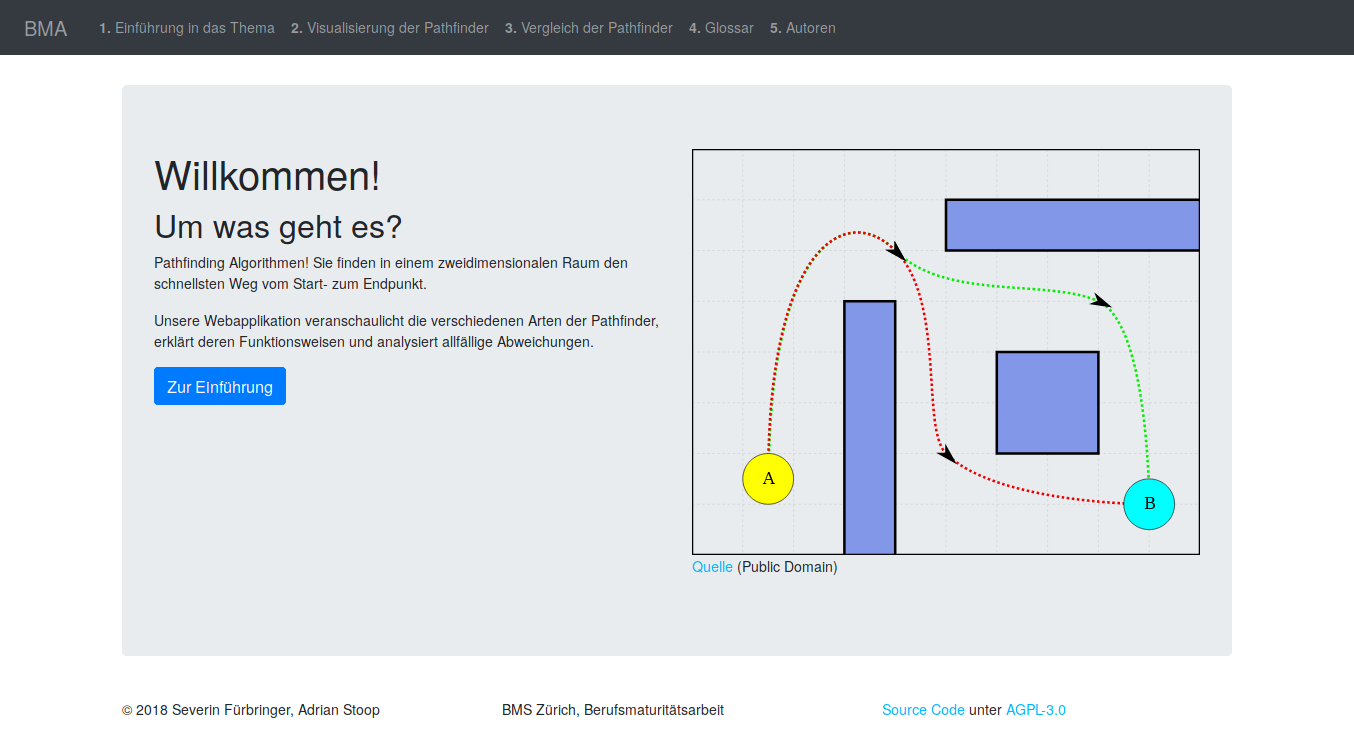
\includegraphics[width=16cm]{0_full}
  \caption[Ein vollständiger Screenshot der Willkommensseite.]{Willkommensseite. Quelle: Eigenleistung}
  \label{fig:welcome_screenshot}
\end{figure}
\subsection{Einleitungsseite}
\begin{figure}[H]
  \centering
  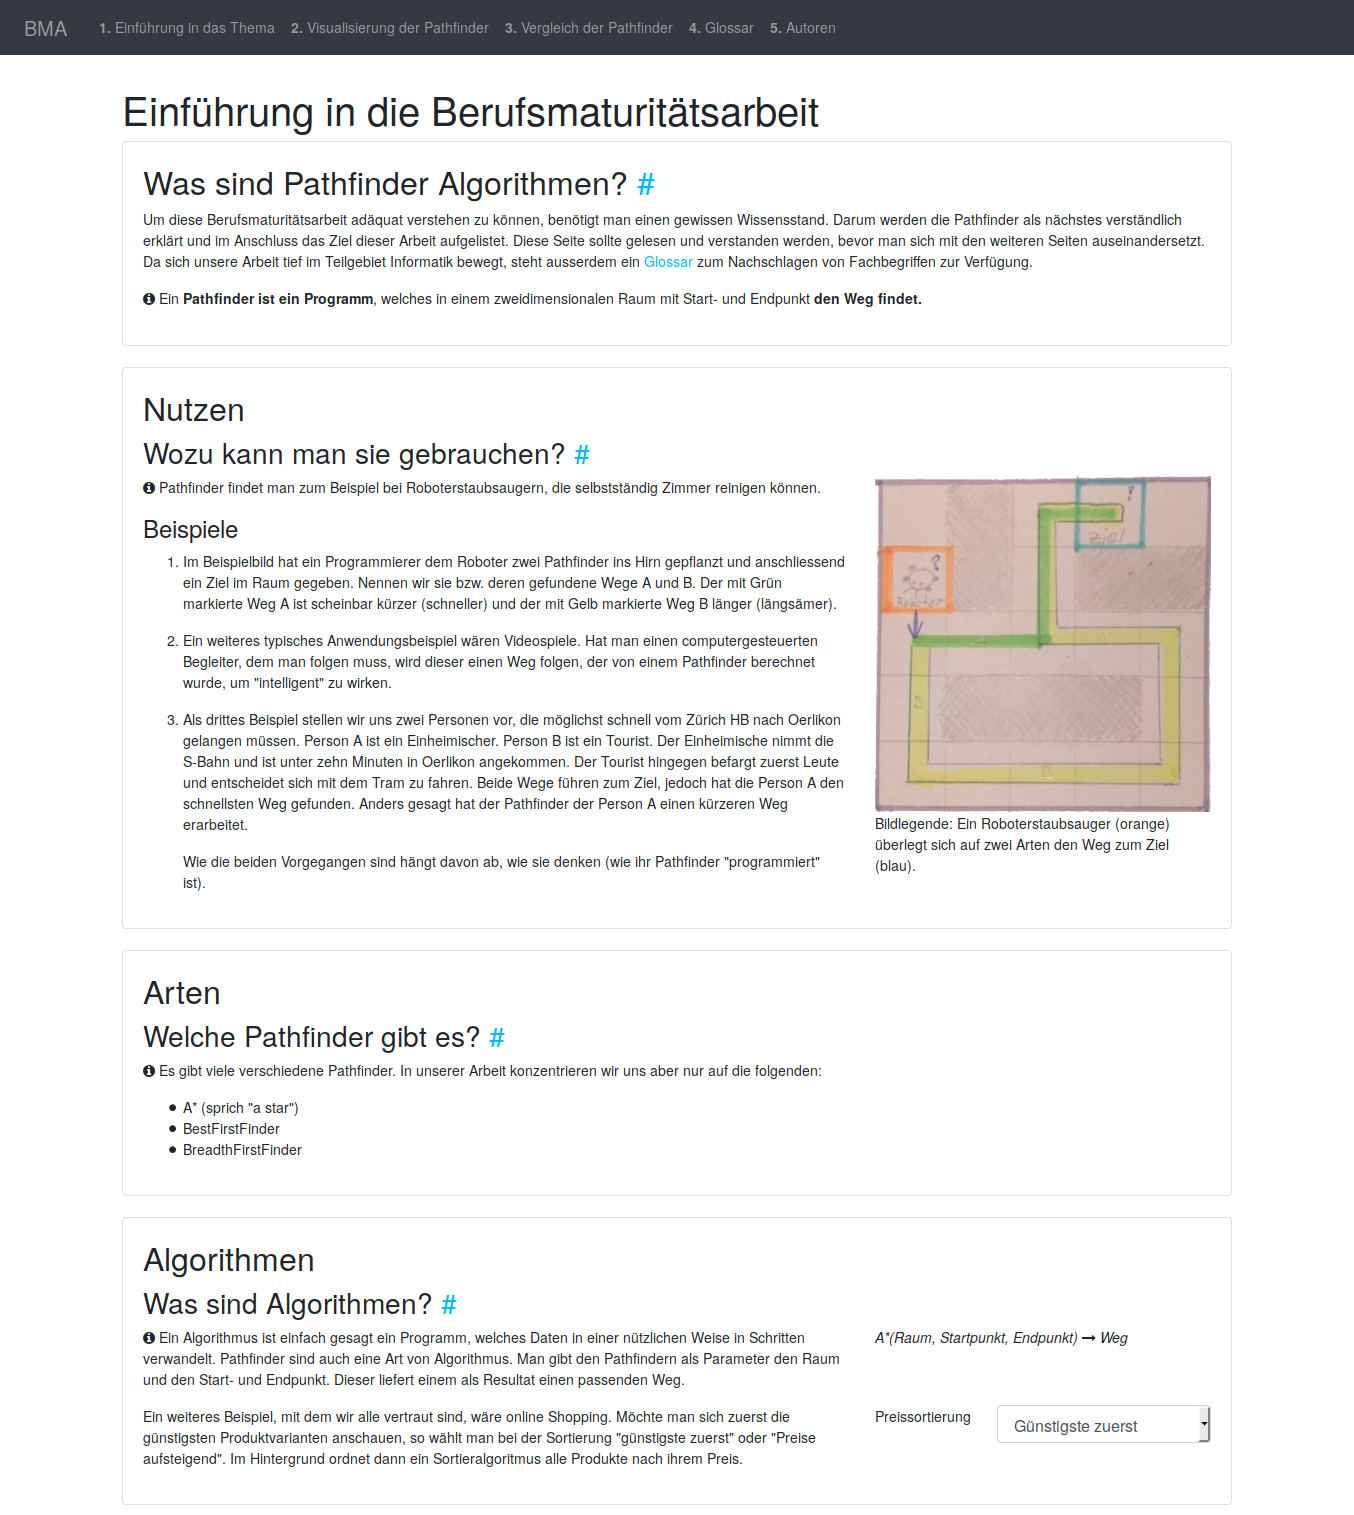
\includegraphics[width=16cm]{1a_full}
\end{figure}
\begin{figure}[H]
  \centering
  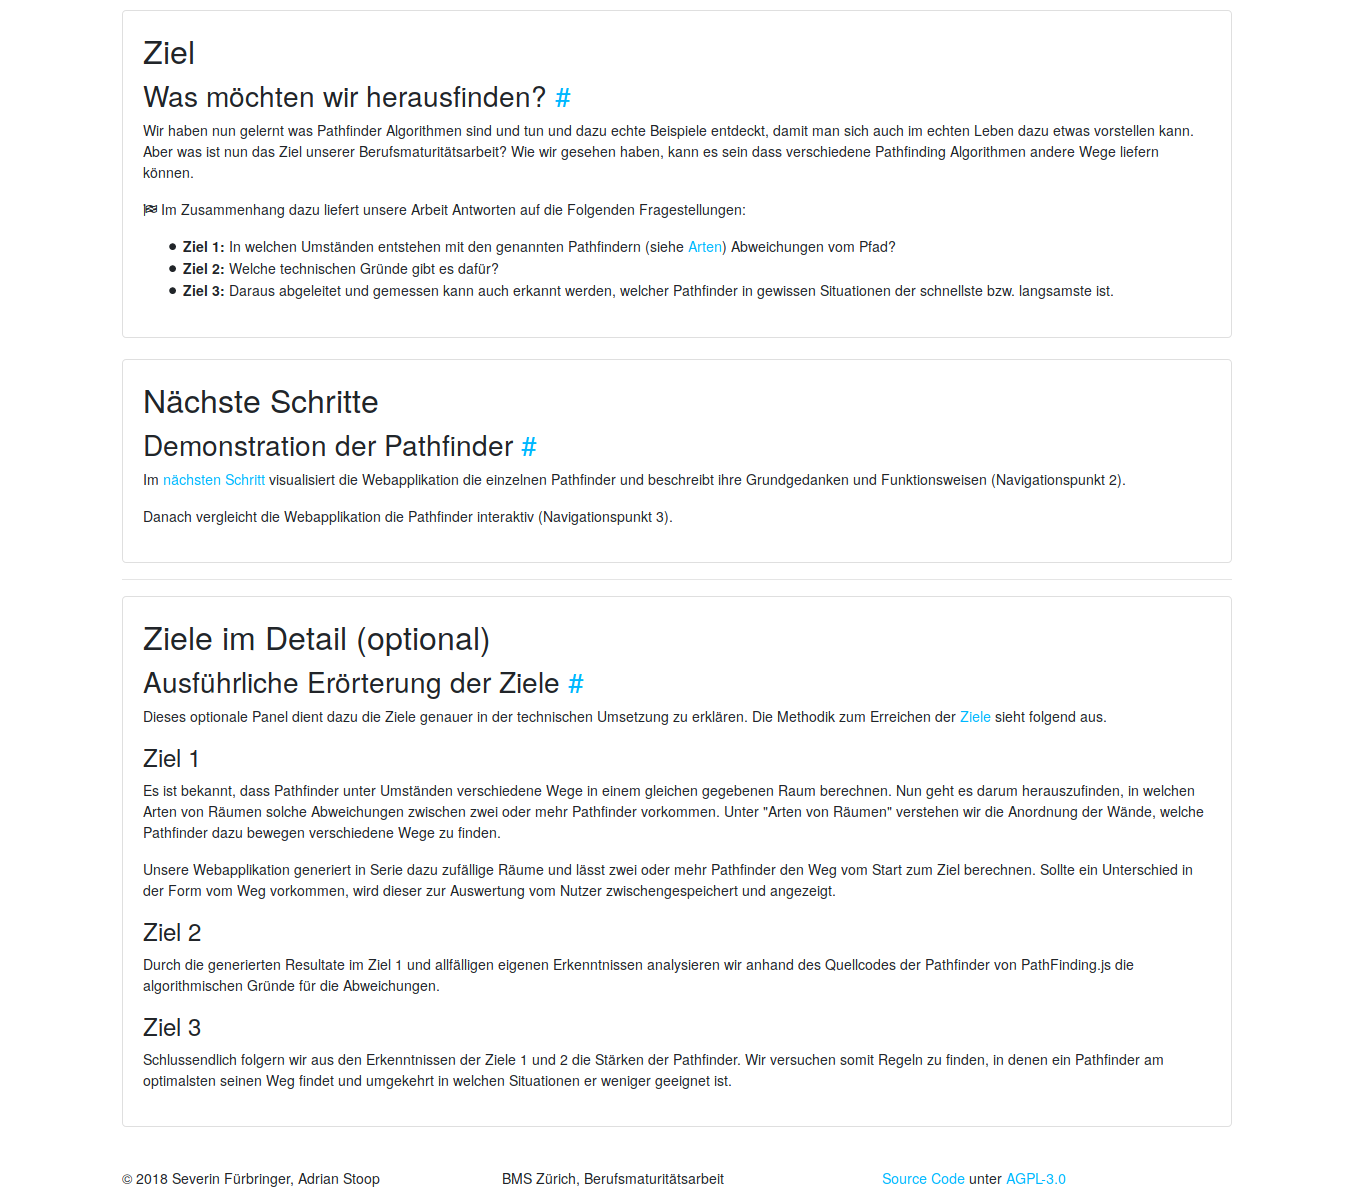
\includegraphics[width=16cm]{1b_full}
  \caption[Ein vollständiger Screenshot der Eileitungsseite.]{Einleitungsseite. Quelle: Eigenleistung}
  \label{fig:intro_screenshot}
\end{figure}
\subsection{Visualisierer}
\begin{figure}[H]
  \centering
  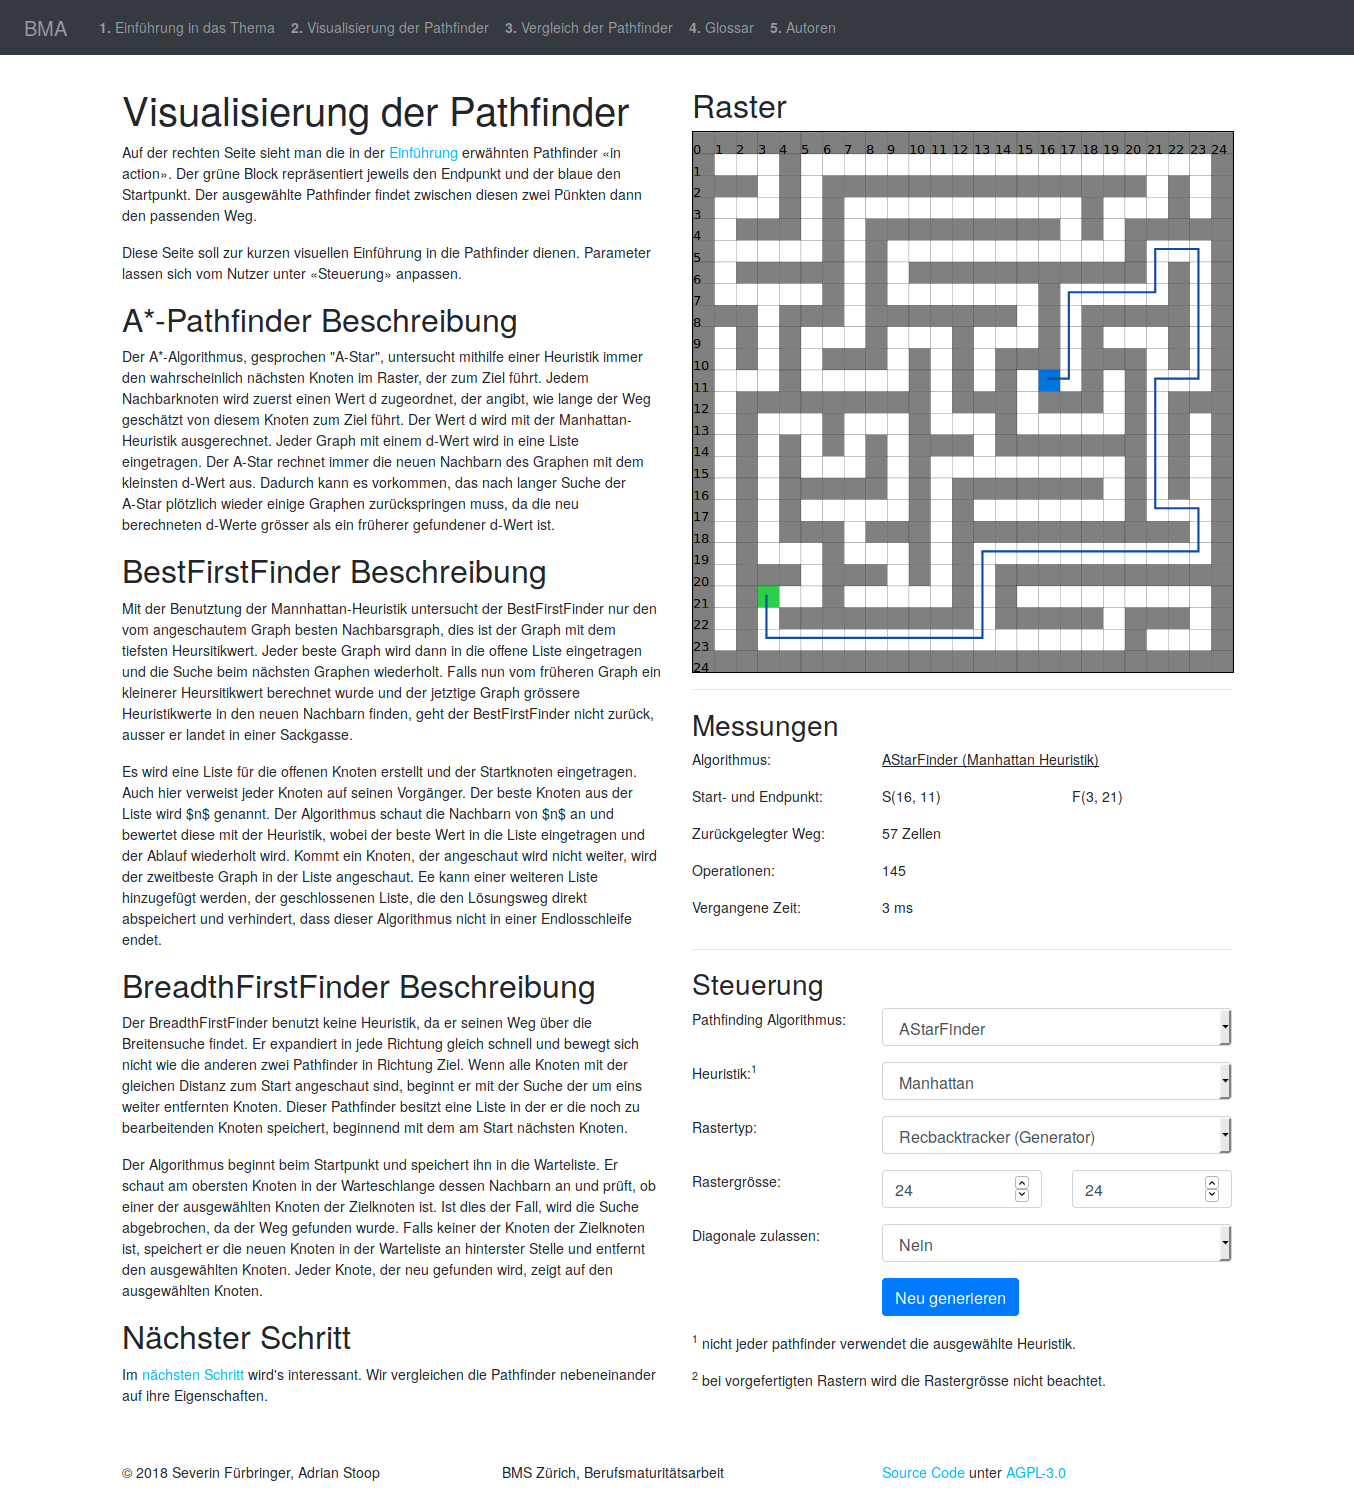
\includegraphics[width=16cm]{2_full}
  \caption[Ein vollständiger Screenshot der Visualisierers.]{Pathfinder-Visualisierer. Quelle: Eigenleistung}
  \label{fig:visualizer_screenshot}
\end{figure}
\subsection{Pathfinder-Vergleicher}
\begin{figure}[H]
  \centering
  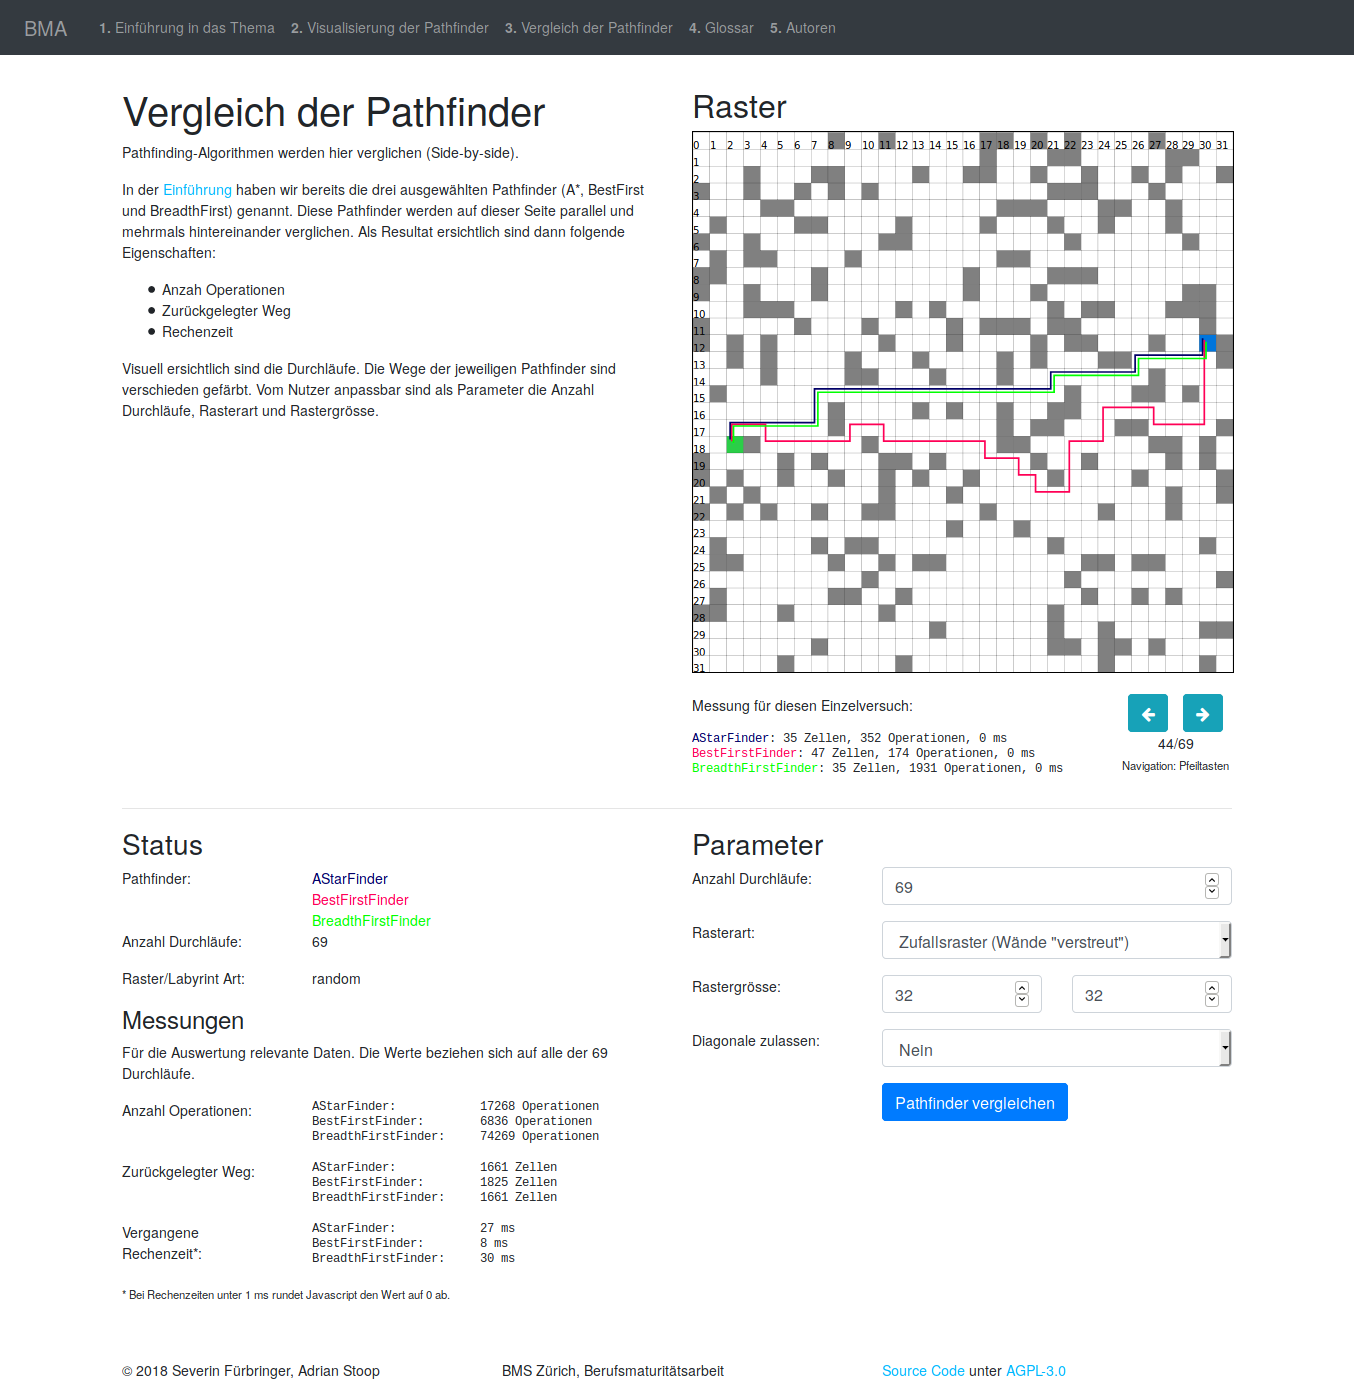
\includegraphics[width=16cm]{3_full}
  \caption[Ein vollständiger Screenshot des Pathfinder-Vergleichers.]{Pathfinder-Vergleicher-Page. Quelle: Eigenleistung}
  \label{fig:comparator_screenshot}
\end{figure}
\subsection{Glossarseite}
\begin{figure}[H]
  \centering
  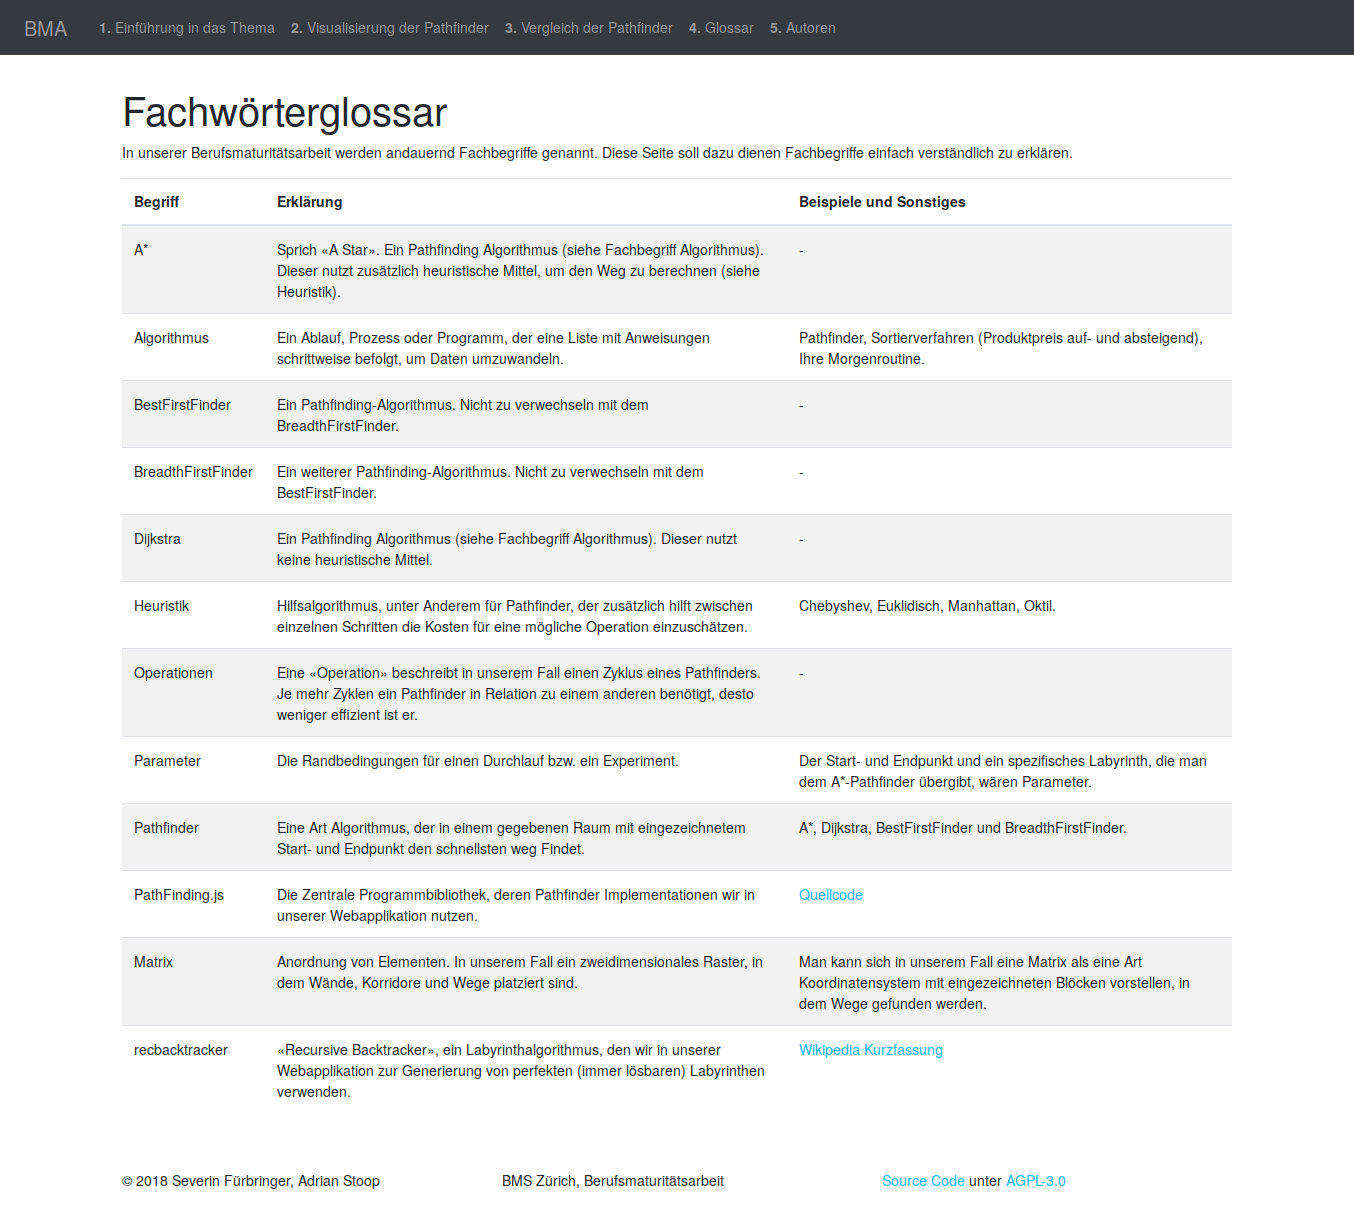
\includegraphics[width=16cm]{4_full}
  \caption[Ein vollständiger Screenshot der Glossarseite.]{Glossarseite. Quelle: Eigenleistung}
  \label{fig:glossary_screenshot}
\end{figure}

\section{Statistiken}
\begin{figure}[H]
  \centering
  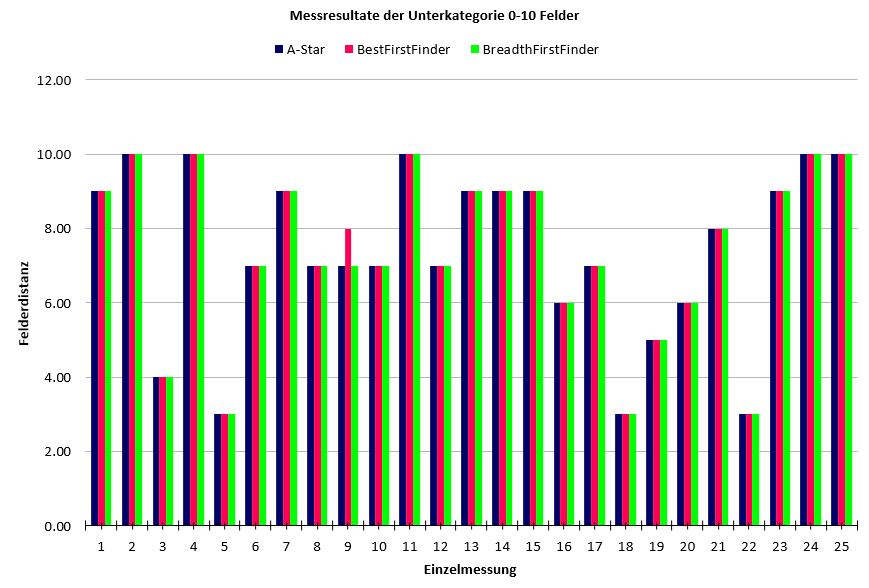
\includegraphics[width=14cm]{statistik_anhang_1}
  \caption[Messresultate der Unterkategorie 0-10 Felder für Felderdistanz.]{Messresultate der Unterkategorie 0-10 Felder für Felderdistanz. Quelle: Eigenleistung}
\end{figure}
\begin{figure}[H]
  \centering
  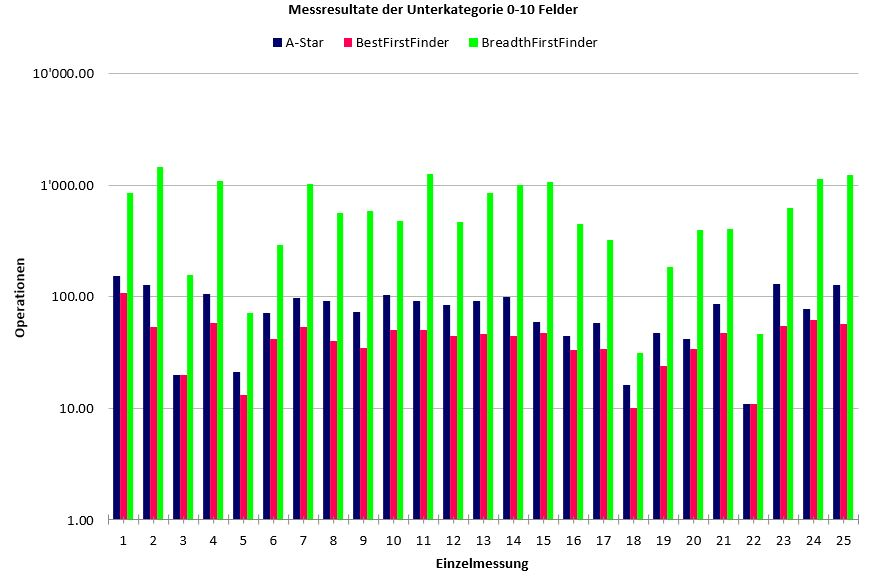
\includegraphics[width=14cm]{statistik_anhang_2}
  \caption[Messresultate der Unterkategorie 0-10 Felder für Operationen.]{Messresultate der Unterkategorie 0-10 Felder für Operationen. Quelle: Eigenleistung}
\end{figure}
\begin{figure}[H]
  \centering
  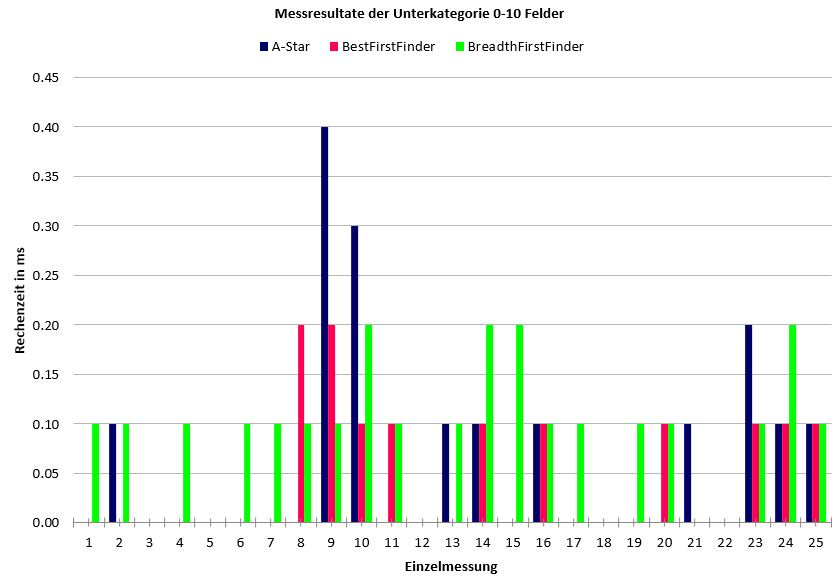
\includegraphics[width=14cm]{statistik_anhang_3}
  \caption[Messresultate der Unterkategorie 0-10 Felder für Rechenzeit in ms.]{Messresultate der Unterkategorie 0-10 Felder für Rechenzeit in ms. Quelle: Eigenleistung}
\end{figure}
\begin{figure}[H]
  \centering
  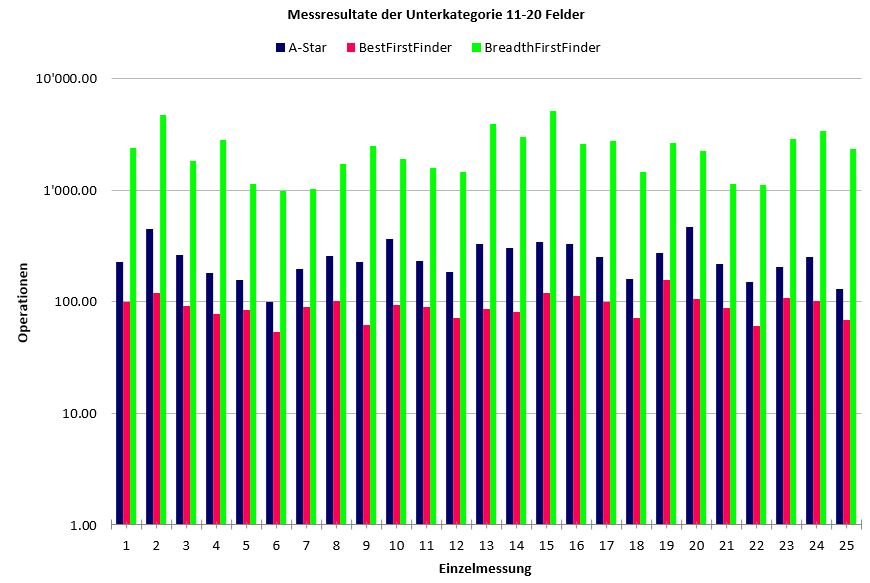
\includegraphics[width=14cm]{statistik_anhang_5}
  \caption[Messresultate der Unterkategorie 11-20 Felder für Operationen.]{Messresultate der Unterkategorie 11-20 Felder für Operationen. Quelle: Eigenleistung}
\end{figure}
\begin{figure}[H]
  \centering
  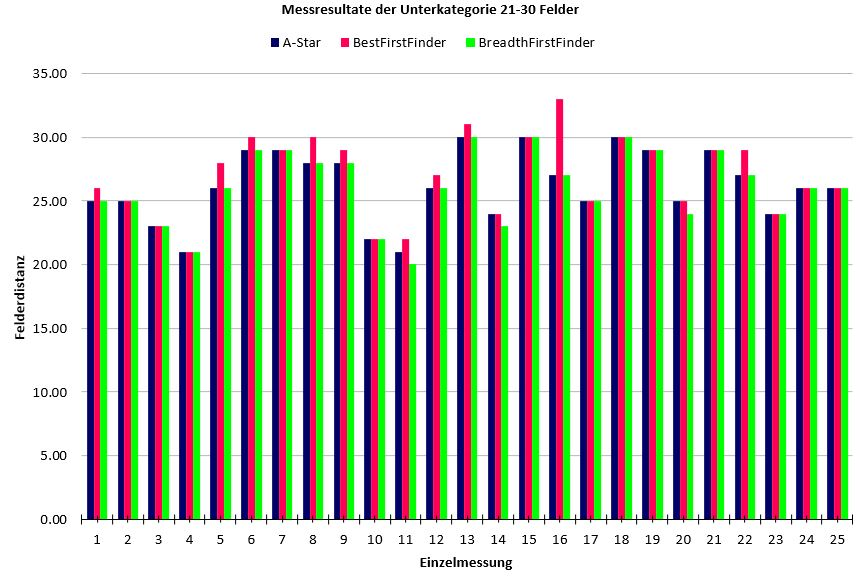
\includegraphics[width=14cm]{statistik_anhang_7}
  \caption[Messresultate der Unterkategorie 21-30 Felder für Felderdistanz.]{Messresultate der Unterkategorie 21-30 Felder für Felderdistanz. Quelle: Eigenleistung}
\end{figure}
\begin{figure}[H]
  \centering
  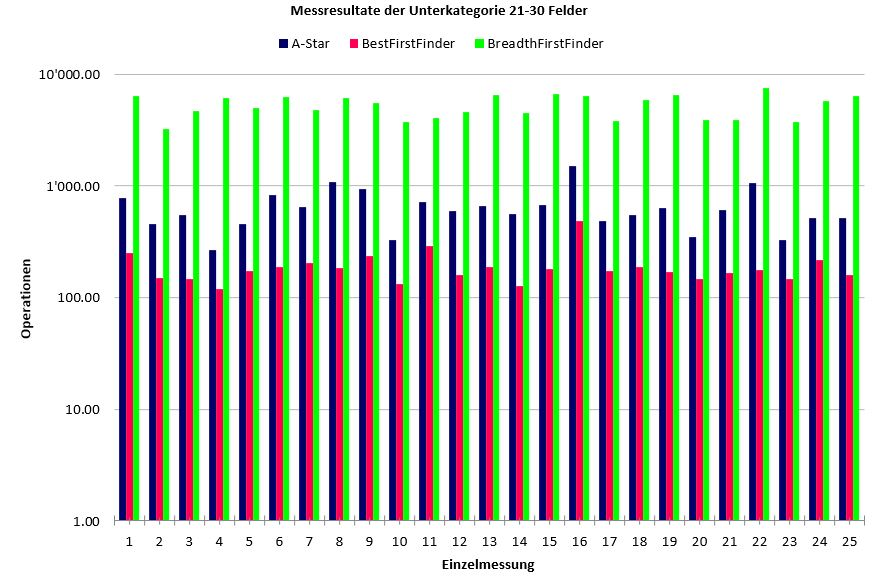
\includegraphics[width=14cm]{statistik_anhang_8}
  \caption[Messresultate der Unterkategorie 21-30 Felder für Operationen.]{Messresultate der Unterkategorie 21-30 Felder für Operationen. Quelle: Eigenleistung}
\end{figure}
\begin{figure}[H]
  \centering
  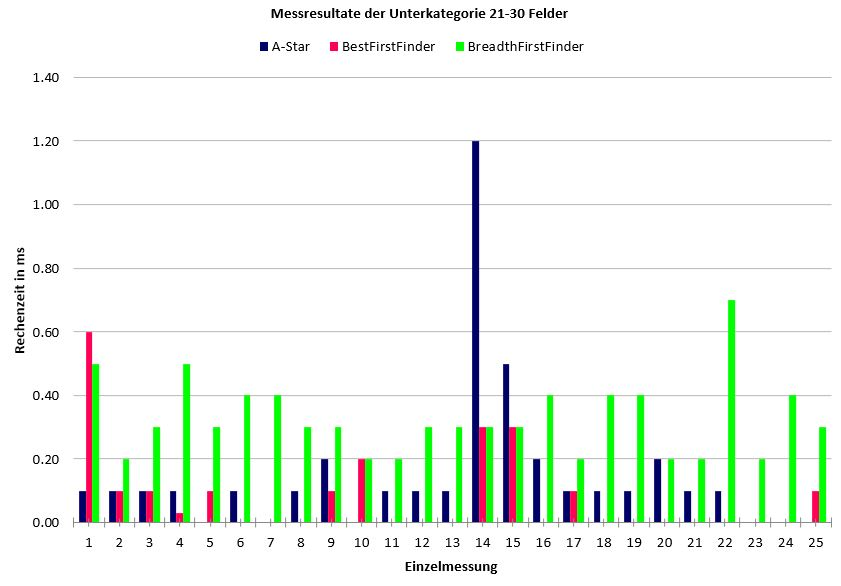
\includegraphics[width=14cm]{statistik_anhang_9}
  \caption[Messresultate der Unterkategorie 21-30 Felder für Rechenzeit in ms.]{Messresultate der Unterkategorie 21-30 Felder für Rechenzeit in ms. Quelle: Eigenleistung}
\end{figure}
\begin{figure}[H]
  \centering
  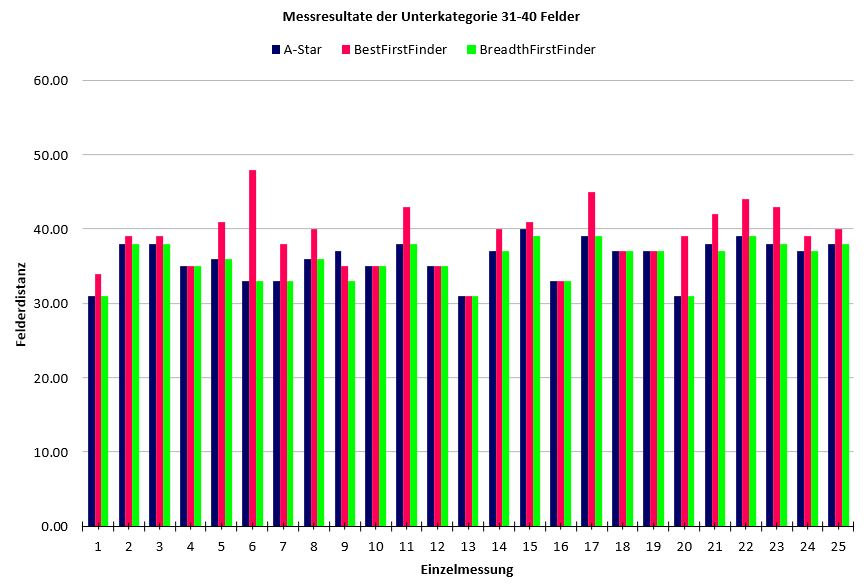
\includegraphics[width=14cm]{statistik_anhang_10}
  \caption[Messresultate der Unterkategorie 31-40 Felder für Felderdistanz.]{Messresultate der Unterkategorie 31-40 Felder für Felderdistanz. Quelle: Eigenleistung}
\end{figure}
\begin{figure}[H]
  \centering
  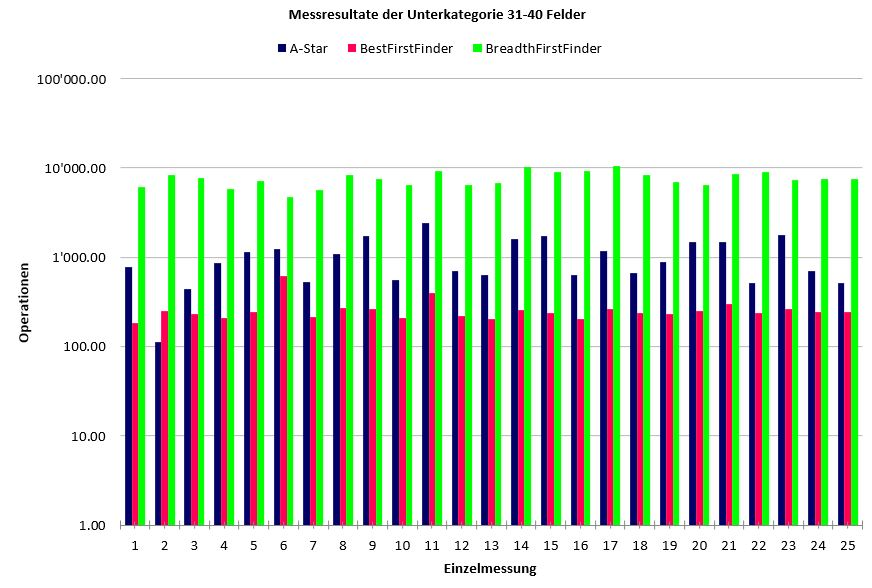
\includegraphics[width=14cm]{statistik_anhang_11}
  \caption[Messresultate der Unterkategorie 31-40 Felder für Operationen.]{Messresultate der Unterkategorie 31-40 Felder für Operationen. Quelle: Eigenleistung}
\end{figure}
\begin{figure}[H]
  \centering
  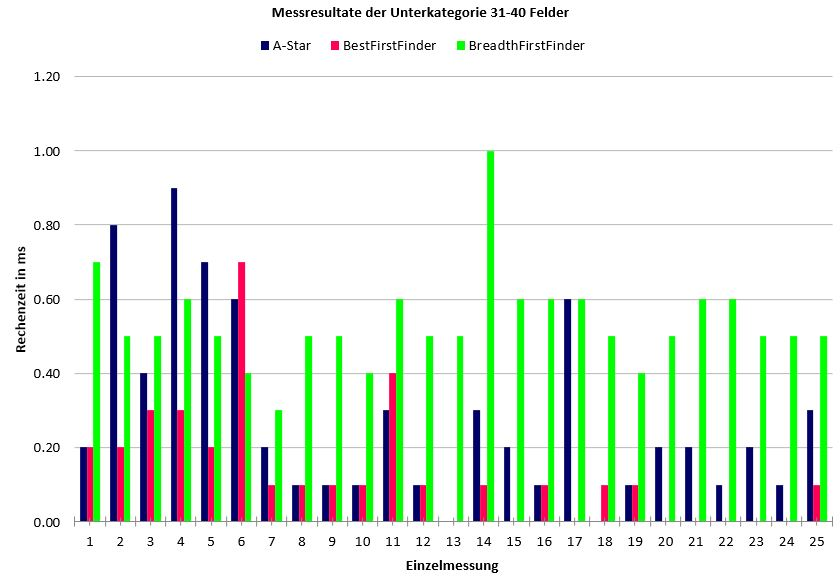
\includegraphics[width=14cm]{statistik_anhang_12}
  \caption[Messresultate der Unterkategorie 31-40 Felder für Rechenzeit in ms.]{Messresultate der Unterkategorie 31-40 Felder für Rechenzeit in ms. Quelle: Eigenleistung}
\end{figure}
\begin{figure}[H]
  \centering
  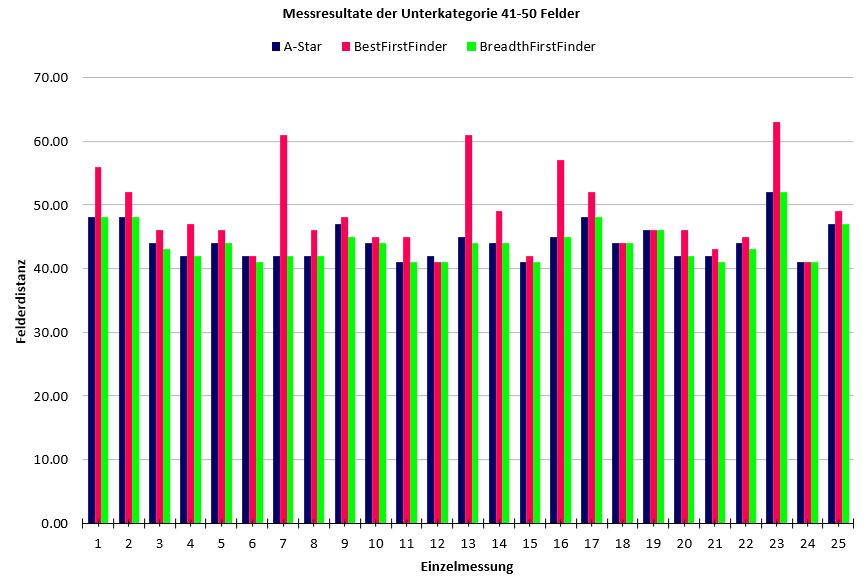
\includegraphics[width=14cm]{statistik_anhang_13}
  \caption[Messresultate der Unterkategorie 41-50 Felder für Felderdistanz.]{Messresultate der Unterkategorie 41-50 Felder für Felderdistanz. Quelle: Eigenleistung}
\end{figure}
\begin{figure}[H]
  \centering
  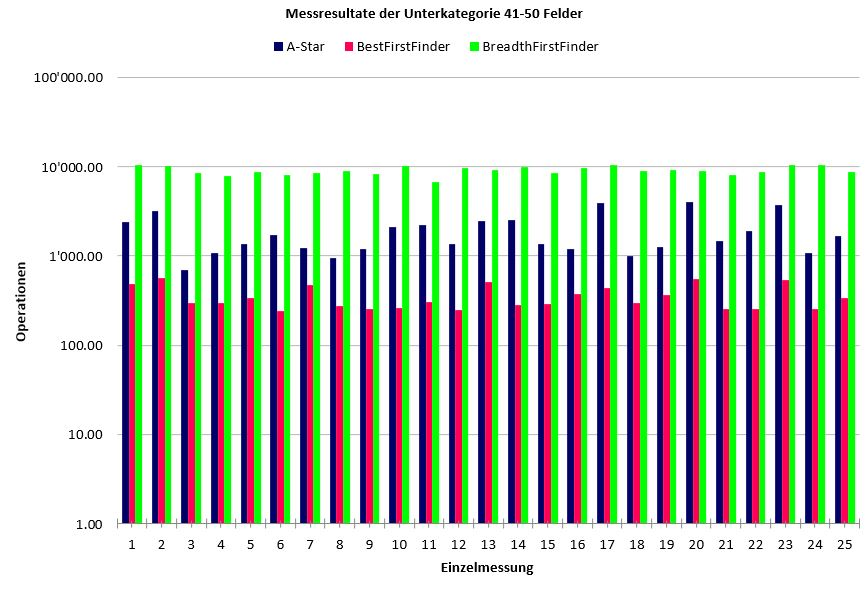
\includegraphics[width=14cm]{statistik_anhang_14}
  \caption[Messresultate der Unterkategorie 41-50 Felder für Operationen.]{Messresultate der Unterkategorie 41-50 Felder für Operationen. Quelle: Eigenleistung}
\end{figure}
\begin{figure}[H]
  \centering
  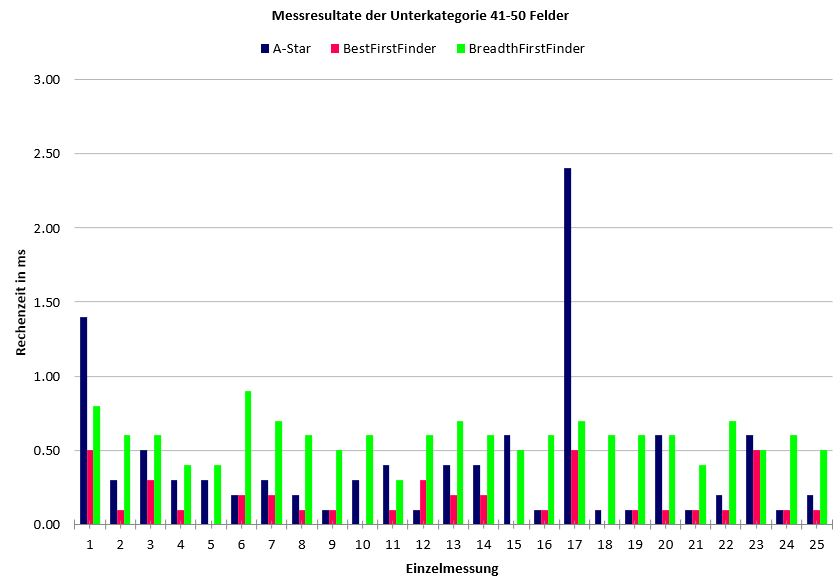
\includegraphics[width=14cm]{statistik_anhang_15}
  \caption[Messresultate der Unterkategorie 41-50 Felder für Rechenzeit in ms.]{Messresultate der Unterkategorie 41-50 Felder für Rechenzeit in ms. Quelle: Eigenleistung}
\end{figure}

\section{Danksagung}
\subsection{Personen}

\subsection{Schriftsetzung}
Die Schriftsetzung wurde durch die freie Software \LaTeX\  und deren Autoren Leslie Lamport et. al. ermöglicht.

\chapter{Glossar}
\section*{Fachwörter- und Begriffsverzeichnis}
In diesem Kapitel werden wichtige Wörter aus der Fachsprache erklärt, die in unserer Arbeit oftmals vorkommen.
\paragraph{A*} Sprich ``A Star''. Ein Pathfinding Algorithmus (siehe Fachbegriff Algorithmus). Dieser nutzt zusätzlich heuristische Mittel, um den Weg zu berechnen (siehe Heuristik).
\paragraph{Algorithmus} Ein Ablauf, Prozess oder Programm, der eine Liste mit Anweisungen schrittweise befolgt, um Daten umzuwandeln.
\paragraph{Back-End} Der Server---mit guten Systemtechnikern rund um die Uhr stellt das Back-End die Website unter einer URL, wie \texttt{bma.fuerbringer.info}, zur Verfügung.
\paragraph{BestFirstFinder} Ein Pathfinding-Algorithmus. Nicht zu verwechseln mit dem BreadthFirstFinder.
\paragraph{BreadthFirstFinder} Ein Pathfinding-Algorithmus. Nicht zu verwechseln mit dem BestFirstFinder.
\paragraph{Dijkstra} Ein Pathfinding Algorithmus (siehe Fachbegriff Algorithmus). Dieser nutzt keine heuristische Mittel und kommt in unserer Arbeit nicht direkt vor.
\paragraph{Front-End} Der Browser---der Teil einer Website oder Webapplikation, den der Benutzer sieht und mit dem er interagiert. In unserem Fall werden die wichtigsten Berechnungen im Front-End verrichtet.
\paragraph{Heuristik} Hilfsalgorithmus, unter anderem für Pathfinder, der zusätzlich hilft zwischen einzelnen Schritten die Kosten für eine mögliche Operation einzuschätzen.
\paragraph{Matrix} Anordnung von Elementen. In unserem Fall ein zweidimensionales Raster, in dem Wände, Korridore und Wege platziert sind.
\paragraph{Operationen} Eine ``Operation'' beschreibt in unserem Fall einen Zyklus eines Pathfinders. Je mehr Zyklen ein Pathfinder in Relation zu einem anderen benötigt, desto weniger effizient ist er.
\paragraph{Parameter} Die Randbedingungen für einen Durchlauf bzw. ein Experiment.
\paragraph{PathFinding.js} Die Zentrale Programmbibliothek, deren Pathfinder Implementationen wir in unserer Webapplikation nutzen.
\paragraph{Pathfinder} Eine Art Algorithmus, der in einem gegebenen Raum mit eingezeichnetem Start- und Endpunkt den schnellsten weg Findet.
\paragraph{recbacktracker} ``Recursive Backtracker, ein Labyrinthalgorithmus, den wir in unserer Webapplikation zur Generierung von perfekten (immer lösbaren) Labyrinthen verwenden. Dieser Algorithmus kommt im Vergleicher nicht zum Zug.
\paragraph{Pseudocode} Definiert einen Algorithmus schriftlich in einer allgemein verständlichen Sprache, damit dieser in beliebigen Programmiersprachen umgesetzt werden kann.
\paragraph{PHP} Eine freie serverseitige Programmiersprache, die seit über zwei Jahrzehnten einen hohen Marktanteil hat.
\paragraph{JavaScript} Nicht zu verwechseln mit Java. Eine clientseitige Programmiersprache, die in jedem Browser integriert ist. Sie wird hauptsächlich zwecks der Interaktivität benutzt. 
\paragraph{Implementieren/Implementation} Im Kontext der Software wird damit die Planung und Entwicklung des Quellcodes bezeichnet.
\paragraph{Pixelmatrizen} Eine Liste mit Pixeldaten, die zum Beispiel bei Computergrafikapplikationen gebraucht wird. Der ``Inhalt'' des Bildschirm kann ganzheitlich in einer Pixelmatrix abgelegt werden.
\paragraph{Prozedural} Beschreibt programme, die schrittartig ablaufen.
\paragraph{Routine} Unter diesem Begriff kann man im Rahmen dieser Arbeit einen Teil eines Algorithmus, einer Funktion oder einer Prozedur verstehen.
\paragraph{Unix und GNU/Linux} Betriebssysteme abstammend vom AT\&T UNIX.
